% Drop-in replacement for plasma_field/sections/pressure_scan_status.tex.
% Figures: copy results/verification/figures/*.pdf into plasma_field/figures/.
\section{Fixed-coil pressure scans and the unresolved derivative}
\label{sec:scanstatus}
A fixed-pressure reconstruction and a pressure derivative are different tests. In the former, one asks whether coils fitted to a finite-pressure target support a nearby equilibrium. In the latter, the coils and signed edge flux are held fixed while pressure changes, and the difference between two nearby equilibria must be resolved. The truncation and equilibrium errors in that difference can exceed the pressure signal even when both equilibria pass conventional convergence tests. This section separates the three ingredients of the comparison: the pressure source, the closed-axis response operator, and the finite-pressure equilibrium solve. The first two are verified independently. The third is shown not to resolve the derivative.

The record uses a newly fitted vacuum coil reference, not the archived finite-pressure coils of the preceding section. Direct Biot--Savart field-line integration determines its closed axis, linear return map, and surrounding vacuum surfaces. The measured signed flux through each traced surface is used as \texttt{PHIEDGE}. The nominal radii $12$, $15$, and $18\,\mathrm{mm}$ correspond to effective flux radii $11.9066$, $14.8678$, and $17.8115\,\mathrm{mm}$; using $\pi B_0a^2$ with the nominal radius would change the flux by $1.5$--$2.1\%$. The candidate coil fit reaches its 600-evaluation budget rather than a stationary optimizer termination. At $18\,\mathrm{mm}$ it nevertheless reproduces the target-axis field and gradient to RMS errors $2.43\times10^{-5}B_0$ and $6.68\times10^{-4}B_0/R_0$. Its direct-field Floquet transform is $-0.212340$ in the laboratory convention and changes by less than $6\times10^{-11}$ relative from 240 to 960 coil segments. The detailed tests below use $a=17.8115\,\mathrm{mm}$ and $p=\alpha p_0(1-s)$ with $p_0=190.3\,\mathrm{Pa}$ and an identically zero current profile. The displacement screen $\alpha\max|\xi|\le0.05a$ gives $\alpha_{\max}=0.17497$, an axis pressure of $33.3\,\mathrm{Pa}$, and volume-averaged $\beta=4.2\times10^{-5}$. For these values \eqref{eq:shiftformula} predicts $\delta R(\phi=0)=2.992\,\mathrm{mm}$ per unit $\alpha$, i.e.\ $0.524\,\mathrm{mm}$ at $\alpha_{\max}$.

\paragraph*{Source.}
The positive-volume current measure of Sec.~\ref{sec:shift} [Eq.~\eqref{eq:shiftcurrent}], placed on the first-order surfaces and integrated by direct Biot--Savart quadrature, reproduces the closed-form on-axis plasma field. The error decreases as $n_\varphi^{-2}$ in the number of toroidal source samples, from $1.43$ at $n_\varphi=101$ to $2.9\times10^{-2}$ at $801$ [Fig.~\ref{fig:sourceoperator}(a)]. After Richardson extrapolation it is $6.8\times10^{-4}$. The on-axis vertical plasma field at $\phi=0$ is $9.26\times10^{-4}\,\mathrm{T}$ per unit $\alpha$, consistent with a Pfirsch--Schl\"uter estimate $\mu_0 j_\parallel a/4$ with $j_\parallel\simeq2\bar\eta R_0|p'|/(\iota_NB_0)$. This checks the matched evaluation against its own current distribution. It does not by itself establish that the truncated current equals the current of a converged equilibrium.

\paragraph*{Closed-axis operator.}
A uniform vertical field $\epsilon B_0\hat z$, which is curl- and divergence-free, was added to the coils and the closed axis re-traced. The periodic solution of the cylindrical variational equation on the traced vacuum axis agrees with the nonlinear difference to first order in $\epsilon$, and to $1.8\times10^{-8}$ after Richardson extrapolation [Fig.~\ref{fig:sourceoperator}(b)]. Its monodromy gives $\iota=0.212340$, matching the direct Floquet value. The near-axis Frenet operator of \eqref{eq:shiftresponse} agrees with the traced operator to $0.22\%$ with either the ideal or the actual coil gradient; this residual is set by the $82\,\mu\mathrm m$ offset between the ideal and traced vacuum axes. Pushing the pressure forcing through the exact traced operator changes $\delta R(0)$ by $0.21\%$. A frozen first-order current added to the coils and traced at finite amplitude gives a shift linear to $2\%$ up to $4\alpha_{\max}$ and sub-linear beyond, reaching $0.87$ of the linear value at $8\alpha_{\max}$ [Fig.~\ref{fig:pressureresponse}(a)].

\paragraph*{Equilibrium solves.}
Table~\ref{tab:pressurescan} and Fig.~\ref{fig:pressureresponse}(b) compare free-boundary VMEX and VMEC2000 solutions at $\alpha_{\max}$. VMEC2000 uses the same runtime deck with a \textsc{makegrid} table of the same coils. Warm continuation in VMEX, as in the earlier record, gives an inward shift of $2.9\%$--$9.8\%$ of theory that depends on the step. Cold starts from the same seed give $+2.0\%$--$2.7\%$, and VMEC2000 cold starts give $+4.2\%$ ($NS=33$) to $+11.5\%$ ($NS=257$) without converging. Raising VMEC2000 to $m=16$, $n=12$ or using a fourfold finer \textsc{makegrid} spacing changes the $NS=65$ value by at most $0.004$; FTOL below about $10^{-13}$ cannot be reached. Above the screen the VMEC2000 response is not analytic in $\alpha$: its ratio to theory grows from $0.07$ to $0.99$ between $\alpha_{\max}$ and $12\alpha_{\max}$, along with the iteration count (1171 to 5165). The $NS=129$ and $m=16$ curves differ from it by up to $27\%$ at $8\alpha_{\max}$. VMEX cold starts remain linear at $1.8\%$--$2.0\%$ of theory up to $12\alpha_{\max}$ and finish in 433--442 iterations at every $\alpha$.

Two measurements expose the cause [Fig.~\ref{fig:pressureresponse}(c)]. First, with FTOL set unreachably small and NITER capped at $10^3$, $4\times10^3$, $1.6\times10^4$, and $6.4\times10^4$, all VMEC2000 states have $F_{\rm sq}\le3\times10^{-12}$, yet the vacuum axis moves by $200\,\mu\mathrm m$ and the response ratio takes the values $0.10$, $0.40$, $0.12$, and $0.34$. Second, every converged free-boundary vacuum axis lies $474$--$536\,\mu\mathrm m$ (VMEC2000, $NS=33$--$257$) or $520$--$688\,\mu\mathrm m$ (VMEX) from the directly traced coil axis. A fixed-boundary solve is within $33\,\mu\mathrm m$. The vacuum-axis error is thus independent of radial resolution and as large as the entire predicted pressure shift at $\alpha_{\max}$. Its origin, which lies outside the pressure source, was not identified. The field of each equilibrium's own current, obtained from Amp\`ere's law on the covariant field and differenced against its vacuum, has an on-axis vertical component of $-0.1$ to $-1.4\times10^{-4}\,\mathrm{T}$ per unit $\alpha$, compared with $+9.26\times10^{-4}\,\mathrm{T}$ from the near-axis current [Fig.~\ref{fig:eqcurrent}(a)]. The differencing floor of this extraction is large, so it corroborates rather than decides. The angle-resolved $m=1$ radial force residual at $s=1/2$ is $5$--$15\,\mathrm{Pa}$ already in vacuum, against an expected Pfirsch--Schl\"uter force of about $3.3\,\mathrm{Pa}$ at $\alpha_{\max}$ [Fig.~\ref{fig:eqcurrent}(b)]. Surface-averaged force balance holds to $0.1$--$1.3\%$ of $p'(s)$.
\begin{table}[t]
\centering
\begin{tabular}{lrrrr}
\toprule
Solver and start&$NS=33$&$65$&$129$&$257$\\
\midrule
VMEC2000 free, cold&$0.042$&$0.068$&$0.071$&$0.115$\\
VMEX free, warm continuation&--&$-0.029$&$-0.005$&--\\
VMEX free, cold&--&$0.020$&$0.023$&--\\
\midrule
Vacuum $R_{\rm axis}-R_{\rm traced}$ ($\mu$m), VMEC2000&$536$&$476$&$479$&$475$\\
Vacuum $R_{\rm axis}-R_{\rm traced}$ ($\mu$m), VMEX cold&--&$688$&$658$&--\\
\bottomrule
\end{tabular}
\caption{Fixed-coil pressure response $\delta R(0)/\delta R_{\rm theory}(0)$ at the screen amplitude $\alpha_{\max}$, $a=17.81\,\mathrm{mm}$, and the offset of each free-boundary vacuum axis from the directly traced coil axis at $\phi=0$. The predicted shift at $\alpha_{\max}$ is $524\,\mu\mathrm m$. No entry is a resolved response coefficient: the sign depends on the restart policy, and the vacuum-axis error exceeds the signal. The analytic amplitude was not adjusted.}
\label{tab:pressurescan}
\end{table}

For a numerical observable $q$, the forward difference $[q_h(\alpha)-q_h(0)]/\alpha$ shows why. If $q_h=q+e_h$, substitution gives
\begin{equation}
 \frac{q_h(\alpha)-q_h(0)}{\alpha}
 =q_1+O(\alpha)+\frac{e_h(\alpha)-e_h(0)}{\alpha}.
 \label{eq:derivativeerror}
\end{equation}
The measurements above give $|e_h|$ of order $200$--$700\,\mu\mathrm m$ for the axis, against $\alpha_{\max}q_1=524\,\mu\mathrm m$, and $e_h$ depends on the iteration history. The axis displacement is a soft mode of the free-boundary energy. A descent solver started from the near-axis seed stops at its force tolerance before that mode relaxes, so the final axis records the seed and the iteration count rather than force balance. A tolerance of $10^{-12}$ on $F_{\rm sq}$ therefore does not resolve a sub-millimetre pressure response at $\beta\sim10^{-4}$. Resolving the derivative requires either a coupled plasma--vacuum tangent $F_UU_\alpha=-F_\alpha$ evaluated at an accepted state, or a free-boundary vacuum axis that agrees with direct tracing to well below $50\,\mu\mathrm m$. Neither is available in the present record. The earlier negative slopes are not an inward physical shift, and no calculation here contradicts \eqref{eq:shiftformula}. The source and operator checks confine the open question to the finite-pressure equilibrium.

\begin{figure}[t]
 \centering
 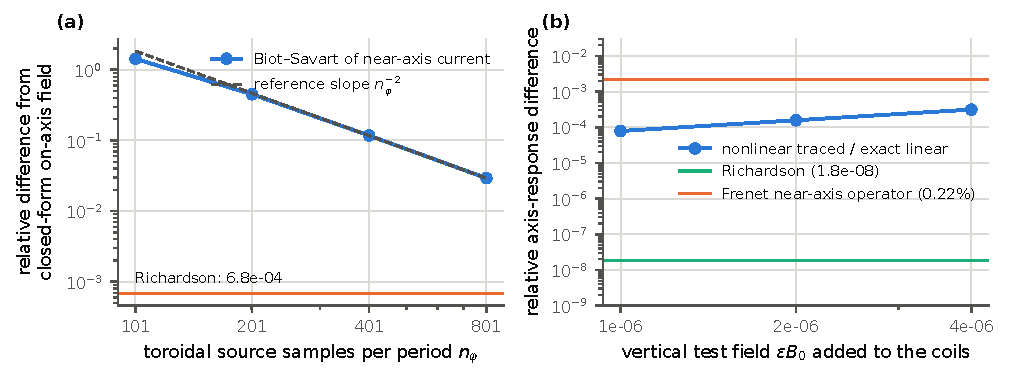
\includegraphics[width=\textwidth]{figures/source_and_operator_verification.pdf}
 \caption{(a) Direct Biot--Savart field of the first-order near-axis current compared with the closed-form on-axis field, against the number of toroidal source samples per period; the horizontal line is the Richardson-extrapolated difference. (b) Closed-axis response to a uniform vertical test field added to the fixed coils: nonlinear traced displacement relative to the exact linear periodic solution on the traced axis, its Richardson extrapolation, and the near-axis Frenet operator.}
 \label{fig:sourceoperator}
\end{figure}
\begin{figure*}[t]
 \centering
 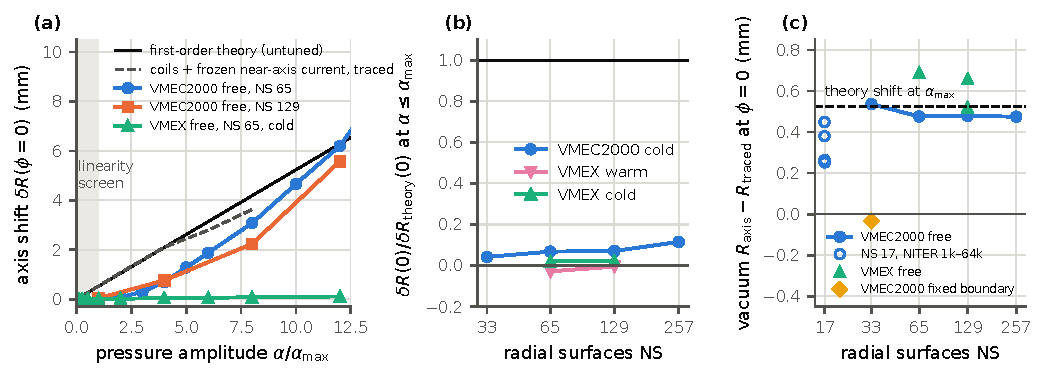
\includegraphics[width=\textwidth]{figures/fixed_coil_pressure_response.pdf}
 \caption{Fixed-coil pressure response at $a=17.81\,\mathrm{mm}$. (a) Axis shift at $\phi=0$ against pressure amplitude: untuned first-order theory, coils plus the frozen first-order current traced directly, and free-boundary VMEC2000 ($NS=65$, $129$) and VMEX (cold) equilibria. The shaded band is the declared linearity screen. (b) Response ratio at $\alpha_{\max}$ against radial resolution and restart policy. (c) Offset of the free-boundary vacuum axis from the directly traced coil axis, including VMEC2000 states with capped iteration counts (open circles) and a fixed-boundary solve; the dashed line is the predicted pressure shift at $\alpha_{\max}$.}
 \label{fig:pressureresponse}
\end{figure*}
\begin{figure}[t]
 \centering
 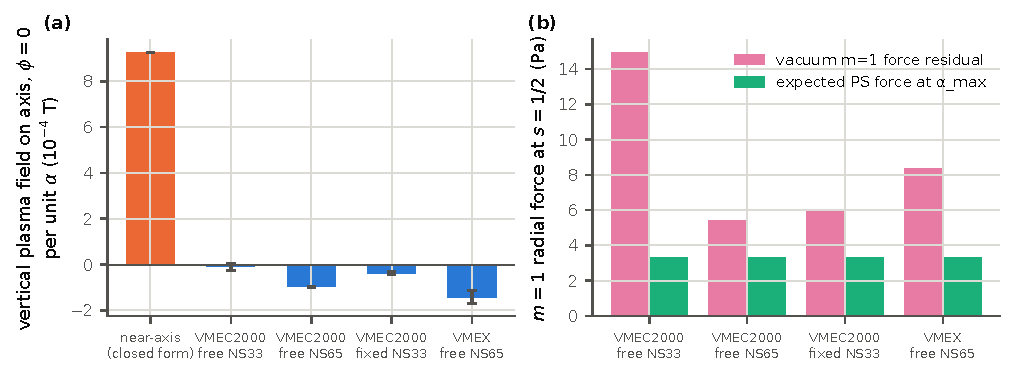
\includegraphics[width=\textwidth]{figures/equilibrium_current_diagnostic.pdf}
 \caption{(a) Vertical plasma field on the vacuum axis at $\phi=0$ per unit $\alpha$: near-axis closed form and the free-space field of each equilibrium's own current at $\alpha_{\max}$, differenced against its vacuum; bars show the change between the two finest toroidal quadratures. (b) Angle-resolved $m=1$ radial force residual of the vacuum solution at $s=1/2$, compared with the expected Pfirsch--Schl\"uter force at $\alpha_{\max}$.}
 \label{fig:eqcurrent}
\end{figure}
